\documentclass{article}

\usepackage[a4paper]{geometry}
\usepackage[ngerman]{babel}
\usepackage[utf8]{inputenc}
\usepackage[T1]{fontenc}
\usepackage{graphicx}
\usepackage{fancyhdr}
\usepackage{amsmath}
\usepackage{xcolor}
\usepackage{float}
\usepackage{hyperref}

\graphicspath{{./images/}}

\pagestyle{fancyplain}
\fancyhf{}
\lhead{\fancyplain{}{Conrad Ferneding, Tobias Ende, Timo Schwabe, Mara Schulke} }
\rhead{\fancyplain{}{\today}}
\cfoot{\fancyplain{}{\thepage}}

\newcommand{\figuresource}[1]{
	\begin{center}Quelle: {#1}\end{center}
}

\begin{document}

\begin{titlepage}
	\begin{center}
		\begin{Large}
			Technische Hochschule Brandenburg \\[1em]
		\end{Large}
		
		IT Sicherheit \\
		Informatik und Medien \\
		Biometrie – Dr.\ Tobias Scheidat
	\end{center}
	
	\vfill

	\begin{center}
		\Large{Teamaufgabe: Offline Handschrift}\\[0.5em]
		\large{Wintersemester 2024}\\[0.25em]
		\large{Abgabetermin \today}
	\end{center}

	\vfill

	\begin{center}
		Tobias Ende – Matr-Nr. 939628 \\
		Timo Schwabe – Matr-Nr. 20229002 \\
		Conrad Ferneding – Matr-Nr. 20246863 \\
		Mara Schulke – Matr-Nr. 20215853 \\
	\end{center}
\end{titlepage}


\tableofcontents

\listoffigures

\newpage

\section{Wenn Sie das FAR/FFR-Fehlerratendiagramm erstellt haben, können Sie nun eine Abschätzung der entstandenen EER (Equal Error Rate) vornehmen. Tun Sie dies und geben Sie das Ergebnis hierfür an.}

Diese Frage wird die Equal Error Rate (EER) bewerten. Das genutzte biometrische System war als Aufgabe 
vorgegeben worden und wird daher nicht ausführlich erläutert werden. Genutzt wurde die Modalität der 
Offline-Handschrift mit zwei verschiedenen Semantiken.

Die EER ergibt sich aus der False Requection Rate (FRR) und der False Acceptance Rate (FAR). Die FRR 
beschreibt die Anzahl der fehlerhaften Ablehnungen im Verhältnis zu der Gesamtanzahl der Versuche. Die FAR 
beschreibt die fehlerhaften Akzeptierungen im Verhältnis zu der Gesamtanzahl der Versuche. Die Stelle, an 
der die FRR und FAR gleich sind, ergibt die EER, welche die Genauigkeit eines biometrischen Systems 
beschreibt. Ein biometrisches System ist ungenau, wenn die EER hoch ist. Die Anzahl der fehlerhaften 
Akzeptierungen und die Anzahl der fehlerhaften Ablehnungen sind dort hoch. Andererseits deutet eine 
niedrige EER auf ein genaueres biometrisches System, da hier die Anzahl der Fehler niedriger ist. Ob das 
biometrische System einen Versuch akzeptiert oder ablehnt, hängt von der berechneten euklidischen Distanz 
zwischen den Enrolment- und Verifikationsvektoren ab.


\begin{figure}[ht]
	\centering
	\begin{minipage}{0.4\textwidth}
		\centering
		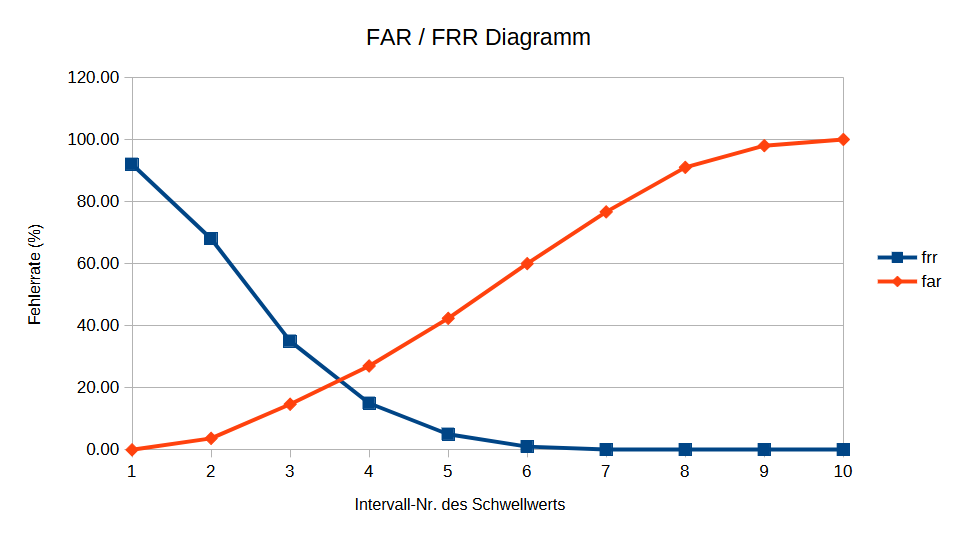
\includegraphics[width=\linewidth]{assets/a-eer}
		\caption{Semantik A - FAR/FRR}
	\end{minipage}%
	\hspace{1em}
	\begin{minipage}{.4\textwidth}
		\centering
		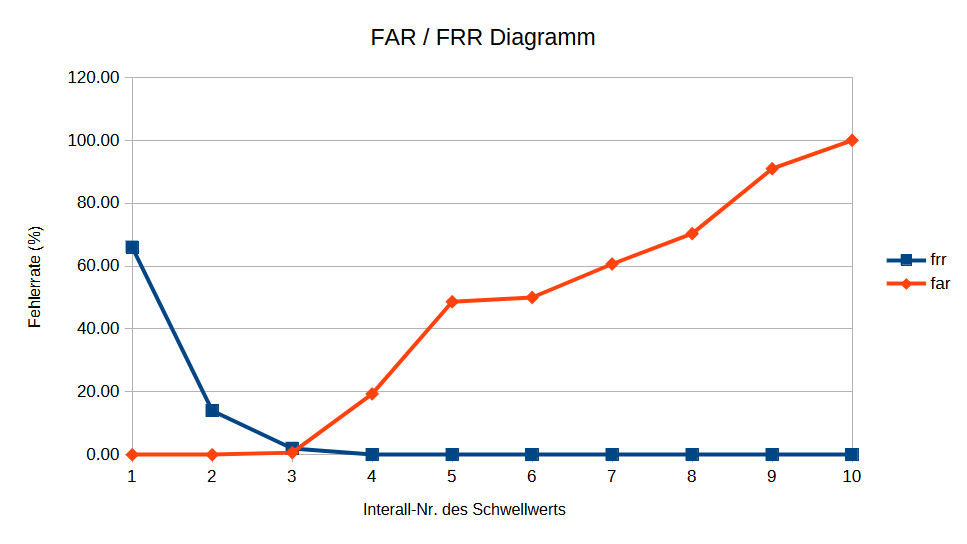
\includegraphics[width=\linewidth]{assets/b-eer}
		\caption{Semantik B - FAR/FRR}
		\label{fig:test2}
	\end{minipage}
\end{figure}

Die EER, welche in Abbildung 1 zu sehen ist, beträgt $\approx22\%$, während die EER aus Abbildung 2,
$\approx2\%$ beträgt. Dass die EER der ersten Semantik höher als die der zweiten Semantik ist, war zu 
erwarten. Bei der ersten Semantik wurden dieselben Schriftzüge geschrieben und bei der zweiten Semantik 
unterschiedlich. Die Merkmalsextraktion bei gleichen Texten lassen weniger Unterschiede zu. Da es sich 
zudem um Zahlen handelte, bei denen z.B. Segmentierung und Schleifen nur begrenzt individualisierbar sind, 
fallen die FAR und die FRR insgesamt höher aus. Wie bereits aus der Aufgabenstellung deutlich wird, 
handelt es sich bei diesen Diagrammen um einen „Zero-Effort“ Fälschungs-Test. (Die Frage, ob diese 
Semantik bereits als blinde Fälschung betrachtet werden kann, wird in den Fragen zwei und vier 
diskutiert.)

Zusätzlich muss an dieser Stelle angemerkt werden, dass lediglich vier Probanden für die Datenerhebung 
genutzt wurden, wodurch die Wirksamkeit dieses biometrischen Systems nicht final widerlegt werden kann.

Generell gibt es keinen Standard, welcher die Sicherheit eines biometrischen Systems anhand dessen EER-
Wertes bewerten kann. Im Zuge dieser Betrachtung wird eine EER von $x < 1\%$ als sicher angesehen, während 
eine EER von $1\% <= x <= 5\%$ als ausreichend betrachtet werden kann. Eine EER von $5\%$ wäre somit 
ausreichend sicher, sollte allerdings nicht in sicherheitskritischen Anwendungen genutzt werden. Solche 
Systeme würden den Komfort des Nutzers über die Sicherheit seiner Daten stellen, da weniger fehlerhafte 
Ablehnungen auftreten bzw. mehr fehlerhafte Anmeldungen zugelassen werden. In einem solchen System würden 
zwei von 100 Versuchen für einen ratenden Angreifer statistischen Erfolg versprechen (FAR). Bei Semantik A 
melden sich alle Nutzer mit demselben Schriftzug an (Enrollment) und erzielen eine 10-Mal höhere EER von 
$22\%$. Diese ist größer als die bereits hohe EER von $2\%$ und dadurch ebenfalls ungenügend. Dadurch das 
bei Semantik A jede Person denselben Schriftzug verwendet, kann die resultierende EER als die Genauigkeit 
der genutzten Merkmale (bei Zahlen) betrachtet werden. Es ist anzunehmen, dass ein Schriftzug aus 
Buchstaben die EER senken wird.

Der Wertebereich der Differenzen der Verifikationen zu den Referenzen ist bei Semantik A kleiner als bei 
der Semantik B. Bei Semantik A liegen alle Distanzen im folgenden Bereich:

$$1,00 <= x <= 10,96$$

Für die Semantik B liegen alle Distanzen im folgenden Bereich:

$$0,31 <= x <= 22.09$$

Die Distanzen des Wertebereichs der Semantik A fallen kleiner aus, wodurch unterschiedliche Personen eine 
größere Wahrscheinlichkeit haben, in einen ähnlichen Wertebereich zu fallen. Ähnlichkeiten der 
Wertebereiche individueller Personen führen zu einer geringeren euklidischen Distanz. Dieser Zusammenhang 
führt bei Semantik 1 zu einer erhöhten FAR/EER. Es ist anzunehmen, dass ein Test mit mehr als vier 
Probanden den finalen Wertebereich vergrößern würde, da extremere Relationen zwischen biometrischen 
Merkmalen auftreten. Ein solcher Test könnte wegen des beschriebenen Zusammenhangs die EER senken.

Bei der Betrachtung der Distanzwerte der FRR- (Intra-Klassen-) Matrizen wird klar, dass nicht alle 
euklidischen Distanzen auf ähnlichem Level gering sind. Es gibt einzelne Ausnahmen, wie z.B. einen Intra-
Klassen-Wert von 6.95 in der Semantik A, welcher die höchste Distanz zum Enrolment aufweist. Ein solch 
hoher Wert wird auch in höheren Intervallen noch abgewiesen. Neben einzelnen Ausnahmen lassen sich durch 
die FRR-Tabelle auch Personen nachweisen, die einen inkonsistenten Schreibstil haben. So hat Person 1 
überwiegend Distanzen im Bereich von $3,29 <= x <= 4,39$, während Person 4 ausschließlich Werte unter 3,29 
aufweist. Person 1 hat einen ungleichmäßigeren Schreibstil als Person 4, was zu einer höheren Rate an 
fehlerhaften Ablehnungen führt. Diese Inkonsequenz im Schreibstil führt dazu, dass die FRR-Kurve der 
ersten Semantik nicht typisch logarithmisch geformt ist, sondern zusätzlich einen Wendepunkt hat

Die Inkonsequenz im Schreibstil lässt sich auch in der zweiten Semantik finden. Allerdings hat diese keine 
Auswirkungen auf diese (wie zuvor festgestellt bessere) Semantik, da der Wertebereich größer ist. Durch 
diese Reichweite fallen die Werte in Intervalle, welche ebenfalls großzügiger sind.

Bei der Betrachtung der FAR- (Inter-Klassen-) Matrizen zeigt sich, dass die festgestellten inkonsistenten 
Schreibstile, scheinbar keine/wenig Auswirkung auf die FAR-Werte haben. Denn obwohl Person 1 in beiden 
Semantiken eine höhere Anzahl an fehlerhaften Ablehnungen aufweist als Person 4, hat Person 4 eine höhere 
Anzahl an fehlerhaften Anmeldungen. Werte im höheren Bereich bei der FRR, schließen somit nicht auf mehr 
fehlerhafte Anmeldungen / ein leichteres Ziel für einen Angriff.

Zusätzlich wird klar, dass sich einige Personen biometrisch ähnlicher sind als andere. So hat Person 2 in 
Semantik B mit keiner anderen Person eine Distanz, die kleiner als 13,67 ist. Im Gegensatz dazu hat Person 
1 zu Person 3 und 4 nie eine Distanz, welche größer als 10,28 ist. Dadurch ergeben sich für Person 1 (im 
Vergleich zu Person 3 und 4) ausschließlich fehlerhafte Anmeldungen in einem Bereich, der für Person 2 
keinen einzigen ergibt. Das Schriftbild von Person 2 ist somit unähnlich dem, von allen anderen. Im 
Gegensatz dazu sind sich die Merkmale der Personen 1, 3 und 4 ähnlicher. Bei Semantik A und B ergibt sich 
durch die biometrische Unähnlichkeit des Schriftbildes von Person 2 zu allen anderen für die FAR ebenfalls 
keine logarithmische, sondern ebenfalls eine Kurve mit Wendepunkt. Die Distanzen liegen vermehrt in 
höheren Intervallen, wodurch die Kurve für die restlichen Werte abflacht. 


\section{Welche weiteren Schritte wäre nötig, um dieses biometrische Verfahren unter dem Einsatz von gezielten Fälschungen zu evaluieren?}

\subsection{Entwicklung der Testprotokolle}

Die Entwicklung eines Testprotokolls für Fälschungsszenarien sollte derart gestaltet werden, dass alle 
relevanten Szenarien systematisch abgedeckt werden. Zunächst sollten Intra-Klassen Tests durchgeführt 
werden. Diese Tests prüfen, wie gut das biometrische System in der Lage ist, authentische Proben einer 
Person korrekt zu erkennen. Dabei werden Verifikationsproben mit den Enrolment-Daten derselben Person 
abgeglichen. Das Ziel dieser Tests ist die Bestimmung der False-Non-Match-Rate (FNMR), welche die 
Häufigkeit beschreibt, mit der authentische Proben fälschlicherweise abgelehnt werden.

Zusätzlich sollten Inter-Klassen Tests mit verschiedenen Angriffsstärken berücksichtigt werden, um die 
Robustheit des Systems gegen Fälschungsversuche zu evaluieren. Diese Tests umfassen:

\begin{itemize}
	\item Blind-Force Angriffe: Bei dieser Angriffsstärke versucht der Angreifer, eine biometrische Probe zu fälschen, ohne Kenntnisse über das Schriftbild oder den Prozess, der zur Erstellung der authentischen Probe geführt hat.
	\item Low-Force Angriffe: Hier hat der Angreifer Zugang zu einem sichtbaren Ergebnis, wie beispielsweise einer Unterschrift, und versucht, dieses nachzuahmen. Es besteht jedoch kein Wissen über den dahinterliegenden Erstellungsprozess, wie etwa Geschwindigkeit, Druck oder Reihenfolge der Bewegungen.
\end{itemize}

\subsection{Erstellung gezielter Fälschungsdaten}

Zur Erstellung gezielter Fälschungsdaten müssen spezifische Angriffstypen berücksichtigt werden, um die Robustheit des biometrischen Systems unter realistischen Bedingungen zu bewerten.
Bei den Blind-Force Daten handelt es sich um Proben, die ohne jegliche Kenntnis des Originals erstellt werden. Der Angreifer versucht, das System zu täuschen, ohne eine Vorlage oder Informationen über das authentische Schriftbild oder den Schreibprozess zu haben.
Bei Low-Force Daten werden auf Grundlage eines sichtbaren Endergebnisses, wie beispielsweise einer Unterschrift, erstellt. Dabei hat der Angreifer keine Kenntnis über den eigentlichen Schreibprozess, wie etwa Bewegungsdynamiken, Geschwindigkeit oder Druck.

\subsection{Implementierung und Durchführung}

Zur Implementierung und Durchführung von Tests sollten mehrere Szenarien berücksichtigt werden, um die Leistungsfähigkeit und Sicherheit des biometrischen Systems zu bewerten. Für den Verifikationstest (Intra-Klassen-Test) werden authentische Proben mit den Enrolment-Daten der gleichen Person abgeglichen. Ziel dieses Tests ist die Messung der False-Non-Match-Rate (FNMR) oder False-Rejection-Rate (FRR), die die intraindividuelle Fehlklassifikation darstellt. Die zuvor erstellten Fälschungsproben werden gegen die Enrolment-Daten der angegriffenen Personen geprüft. Ziel dieser Tests ist die Messung der False-Match-Rate (FMR) oder False-Acceptance-Rate (FAR) für die jeweiligen Angriffsszenarien (FMRBlind, FMRLow-Force).

\subsection{Analyse der Ergebnisse}

Zur Bewertung der Testergebnisse werden folgende Punkte analysiert. Der Punkt, an dem die False-Match-Rate 
(FMR) und die False-Non-Match-Rate (FNMR) gleich sind ist die Equal-Error-Rate (EER). Für die 
Angriffsszenarien Blind und Low-Force wird jeweils eine separate EER berechnet, um die Robustheit des 
Systems gegenüber unterschiedlichen Angriffsstärken zu bewerten. Durch den Vergleich der Fehlerraten wird 
dann analysiert, wie sich die Falscherkennungsraten zwischen Blind- und Low-Force-Angriffen verändern. Ein 
Anstieg der FMR von Blind- zu Low-Force-Angriffen kann auf Schwachstellen im System hinweisen. 

\subsection{Bewertung und Optimierung des Systems}

Auf Grundlage der Testergebnisse können gezielte Maßnahmen zur Verbesserung des biometrischen Systems 
ergriffen werden. Zum einen kann eine Verbesserung der Algorithmen vorgenommen werden. Es sollten 
spezifische Fälschungserkennungsmethoden entwickelt werden, die gezielt auf die Schwachstellen des Systems 
bei Blind- und Low-Force-Angriffen eingehen. Außerdem kann die Systemschwelle erhöht werden. Die Anpassung 
der Entscheidungsschwellen kann dazu beitragen, die Falscherkennungsrate bei Angriffen zu verringern, ohne 
die Benutzerfreundlichkeit zu beeinträchtigen. Zuletzt können mehrere Merkmale kombiniert werden. Die 
Integration zusätzlicher biometrischer Eigenschaften wie Schreibdruck oder Schreibgeschwindigkeit kann die 
Sicherheit des Systems erhöhen und es widerstandsfähiger gegen gezielte Fälschungen machen.

\subsection{Iterative Tests und Validierung}

Nach der Optimierung des biometrischen Systems sollten erneut Tests durchgeführt werden, um die Wirksamkeit der vorgenommenen Anpassungen zu validieren.

\begin{itemize}
	\item Langzeitbeobachtungen: Es ist wichtig zu überprüfen, ob die Verbesserungen des Systems über einen längeren Zeitraum hinweg stabil und nachhaltig bleiben. Dies hilft, potenzielle Schwächen oder Verschlechterungen in der Leistung frühzeitig zu erkennen.
	\item Cross-Validation: Die Ergebnisse sollten auf unterschiedliche Benutzergruppen und Nutzungsszenarien übertragen werden, um sicherzustellen, dass die Verbesserungen universell anwendbar sind und nicht nur unter spezifischen Bedingungen funktionieren.
\end{itemize}

\subsection*{Ausschluss von Zero-Effort}

\begin{quote}
	Ein erwähnenswerter Angriff, der aber nicht gezielt für dieses Szenario relevant ist, ist der Zero-
	Effort/Random-Angriff. Das ist ein Angriff, dessen Ziel es ist, ohne gezielte Fälschungen, also 
	zufälligen Versuchen, das System zu täuschen. Ein Zero-Effort Fälschungstest ist also ein Test, bei 
	dem zufällige Proben gegen die Enrolment-Daten anderer Personen geprüft werden. Das Ziel dieses Tests 
	ist die Bestimmung der False-Match-Rate (FMR) oder False-Acceptance-Rate (FAR) für zufällige 
	Übereinstimmungen.	
\end{quote}

\section{Welche Rahmenvorgaben-/ annahmen sollten dabei Berücksichtigung finden}

Insbesondere die technische Infrastruktur und die Umgebung der Erfassung der Daten müssen für alle Probanden gleich sein, um vergleichbare Resultate zu erzielen.

\subsection{Umgebung}

Die Schriftproben sollten so erhoben werden, dass kein anderer Proband die Erfassung beobachten kann, zum 
Beispiel durch einen Sichtschutz. So können Brute-Force Angriffe früh unterbunden werden.
 
\subsection{Erfassung}

Offline Handschriften können über verschiedene technische Verfahren erhoben werden. Im Folgenden werden 
zwei Beispiele 

\subsubsection{Scanner}

Eine Möglichkeit bieten handelsübliche Dokumentenscanner. Sie beleuchten die Schriftprobe und erfassen das 
reflektierte Licht der Schrift. Wichtig hierbei ist eine hohe Auflösung des Geräts, damit das Schriftbild 
detailliert erfasst werden kann und auch feine Striche, kleine Punkte oder Lücken in der Schrift erkannt 
werden können.

Scanner haben den Vorteil, dass sie unter immer gleichen Bedingungen arbeiten. Die Beleuchtung und 
Auflösung ändern sich nicht. Dafür sind sie aber nicht mobil und brauchen Platz. Sie werden ungenau, wenn 
die Schriftproben beschädigt oder geknittert sind.

\subsubsection{Digitalkameras}

Alternativ können Digitalkameras zur Erfassung von Schriftproben verwendet werden. Hierbei spielt die 
Auflösung ebenfalls eine Rolle. Eine bessere Auflösung bietet mehr Details. Des Weiteren spielt das 
verwendete Objektiv eine große Rolle, um Verzerrungen zu verhindern. Der Vorteil von Digitalkameras ist, 
dass sie in vielen verschiedenen Größen existieren. Sie sind mobil und nicht stationär. Ein Nachteil ist, 
dass es schwer ist, identische Voraussetzung für die Erfassung zu gewährleisten, da Licht, Winkel und 
Abstand zur Schriftprobe leicht verändert werden können.

Jeder Sensor muss entsprechend kalibriert und gewartet werden, damit identische Bedingungen bei der
Erfassung herrschen.

\subsection{Speicherung}

Eine sichere und effiziente Speicherung spielt eine tragende Rolle. Damit später eine präzise Analyse der 
erfassten Daten möglich ist, müssen die Rohdaten in einem verlustfreien Format gespeichert werden. 
Relevante Metadaten, wie Informationen zum Sensor und den Probanden sind ebenfalls zu erheben, damit bei 
Fehlern ein entsprechendes Troubleshooting erfolgen kann.

Da es sich um biometrische, und damit besonders schützenswerte Daten handelt, ist ein Zugriffs- und 
Berechtigungssystem nötig. Dadurch kann der Zugriff auf die Daten sowohl eingeschränkt, als auch 
nachvollzogen werden. Außerdem müssen biometrische Daten immer ausreichend verschlüsselt gespeichert und 
übertragen werden.

\section{Beschreiben Sie ein Protokoll für die hierfür erforderliche Datenerhebung}

\subsection{Vorbereitung der Datenerhebung}

\subsubsection{Definition der Zielsetzung}

Das Ziel dieser Datenerhebung ist die Evaluierung der Fälschungssicherheit unseres biometrischen Systems 
im Hinblick auf die, handschriftliche erfassten, Semantiken:

\begin{itemize}
	\item \textbf{Semantik A}: Numerische, 5-stellige PIN (78402)
	\item \textbf{Semantik B}: Der Geburtsort jedes Probanden
\end{itemize}

Es wird ein besonderer Fokus auf zwei gezielte Angriffe gelegt:
Blind-Force: Angriffe basierend auf visuellen Vorlagen.
Low-Force: Angriffe mit Zugriff auf eine authentische Verifikationsprobe

\subsubsection{Auswahl der Probanden}

Idealerweise 50–100 Probanden (angenommen es handelt sich um ein echtes biometrisches System) bzw. 2-4 (in 
dem Rahmen dieses Moduls)

Probanden sollten ein unterschiedliches Alter, Geschlecht und einen unterschiedlichen Schreibstil haben, 
um eine ausreichende Intra-Class-Variabilität zu gewährleisten.

Eine schriftliche Einwilligung gemäß Datenschutzrichtlinien (z. B. DSGVO) ist einzuholen.

\subsubsection{Technische Infrastruktur}
Es müssen abhängig von der Probanden-Anzahl mehrere Schreibtabletts oder Touchscreens zur Datenerfassung bereitgestellt werden.
Speicherung der Proben als Bild- oder Vektordaten.
Umgebung: Einheitliche Bedingungen (z. B. Beleuchtung, Schreibfläche).

\subsection{Durchführung der Datenerhebung}

Da diese Datenerhebung ausschließlich auf gezielte Angriffe bezogen ist, werden Enrolment- und 
Verifikationsproben nicht erneut erhoben. Eine Variante (falls mehr authentische Probanden gefordert sind) 
könnte sein, diese ebenfalls zu erheben, da der logistische Aufwand fast identisch ist.

\subsubsection{Erhebung der Fälschungsproben}

\subsubsection*{Blind-Force-Angriffe}

\begin{flushleft}
	\textbf{Semantik A}: Angreifer erhalten die Pin und erfassen 5 Fälschungsproben für diese\\
	\textbf{Semantik B}: Angreifer erstellen für jeden authentischen Nutzer 5 Fälschungsproben	
\end{flushleft}


\subsubsection*{Low-Force-Angriffe}

\textbf{Semantik A und B}: Angreifer erhalten für jeden Nutzer (4 in unserem Fall) Zugriff auf Bilder der 
authentischen Proben und erfassen jeweils 5 Fälschungsproben!

\subsection{Verarbeitung der Daten}

\subsubsection{Qualitätssicherung}

\begin{flushleft}
	\textbf{Semantik A}: Prüfung auf numerische Vollständigkeit und Klarheit\\
	\textbf{Semantik B}: Prüfung auf Lesbarkeit und Textvollständigkeit, sowie Übereinstimmung des Geburtsortes mit dem authentischen.	
\end{flushleft}

\subsubsection{Anonymisierung}

Um eine DSGVO-konforme Verarbeitung von Probandendaten zu gewährleisten, werden alle Referenzen zu 
personenbezogenen Daten durch pseudonymisierte IDs ersetzt. Somit lassen sich Angreifer unterscheiden, es 
gibt allerdings keine Möglichkeit, einen Rückschluss auf den tatsächlichen Probanden zu ziehen.

\subsubsection{Datenaufteilung}

Die erhobenen Daten werden in zwei Gruppen unterteilt (angenommen es handelt sich um eine große Anzahl an Probanden):

\begin{enumerate}
	\item Trainingsdaten, die für eine weitere Systemoptimierung verwendet werden können
	\item Testdaten, die für eine Evaluation des biometrischen Systems genutzt werden können
\end{enumerate}

\subsection{Evaluierung der Angrifftests}

Um die Evaluierung des Systems gegen die zwei Arten von Angriffen durchzuführen werden sogenannte Angrifftests durchgeführt:

\subsubsection{Blind-Force-Angrifftests}

In den Blind-Force-Angrifftests werden:

\begin{enumerate}
	\item In Semantik A, pro Angreifer 5 Verifikationsversuche unternommen und die FAR berechnet
	\item In Semantik B, pro Nutzer  5 Verifikationsversuche unternommen und die FAR berechnet
\end{enumerate}

Die unterschiedliche Natur der beiden Semantiken führt bei Blind-Force-Angriffen dazu, dass es 
unterschiedlich viele Angriffe für Semantik A \& B gibt.

\subsubsection{Low-Force-Angrifftests}

In den Low-Force-Angrifftests werden:

\begin{enumerate}
	\item In Semantik A, pro Angreifer und Proband Verifikationsversuche unternommen und die FAR berechnet
	\item In Semantik B, pro Angreifer und Proband, Verifikationsversuche unternommen und die FAR berechnet
\end{enumerate}

\subsection{Dokumentation und Auswertung}

\subsubsection{Fehleranalyse}

In die bestehenden Diagramme aus Aufgabe 1) für FAR/FRR können nun, für jede Semantik, zwei weitere Graphen eingezeichnet werden:

\begin{enumerate}
	\item Blind-Force-FAR – Die Acceptance-Rate von Angreifern, die Zugriff auf das geheime Wissen (bspw. Pin/Ort respektive) hatten, aber kein Beispiel für die Handschrift hatten.
	\item Low-Force-FAR – Die Acceptance-Rate von Angreifern, die Zugriff auf authentische offline Verifikationsdaten von authentischen Probanden hatten.
\end{enumerate}

Des Weiteren könnte eine Fehleranalyse dieser Charakteristiken erfolgen:

\begin{enumerate}
	\item Schriftproben haben (bspw. wie schneiden Schreibschrift vs. Druckschrift ab?) 
	\item Inhalte haben (bspw. wie schneiden kurze Städtenamen vs. lange ab?)
\end{enumerate}

um Rückschlüsse auf das Verhalten der Merkmalsextraktion zu erhalten.

\subsubsection{Berichterstellung}

Wie oben bereits beschrieben, müssen Semantik A und B separat ausgewertet werden. Die eingezeichnete FAR 
der verschiedenen Angriffe in den Diagrammen kann daraufhin genutzt werden, um einen verbesserten 
Schwellwert oder Änderungen am biometrischen System vorzuschlagen.

\subsubsection{Optimierung}

Letztlich sollten Anpassungen des Systems vorgenommen werden, um die Robustheit gegen gezielte Fälschungen 
zu erhöhen. Nach erfolgten Anpassungen kann das System mit den hier erstellten Angrifftests erneut 
getestet und ausgewertet werden, um eine Verbesserung bzw. Verschlechterung festzustellen.

\end{document}
